\documentclass[12pt]{article}

% preamble begins
\title{CS261 Final Report}
\author{Team 29 \\\\ \textbf{Sylvester Cardorelle},\textbf{Tudor Cismarescu}, \textbf{Ollie Madelin},\\
\textbf{Josh Footman}, \textbf{Joseph Parkins}, \textbf{Anil Kiral}}
\date{March 2017}
\usepackage{graphicx}
\usepackage{listings}
\usepackage{scrextend}
\usepackage{titlesec}
\usepackage{float}
\usepackage[margin=0.8in]{geometry}
%preamble ends


%content begins
\begin{document}
\begin{titlepage}
\maketitle
\centering
\vfill
\vfill

\includegraphics[width=7cm]{logo.png}
\vfill
\vfill
\thispagestyle{empty}
\end{titlepage}
\tableofcontents
\newpage
\section{Installation Guide/System Requirements }
  Before using the application both NodeJS and Java JDK needs to be running on the server.
  These can be installed using the following terminal commands.
	\subsection{Setup}
		\subsubsection{Node}
    \begin{figure}[H]
    \centering
    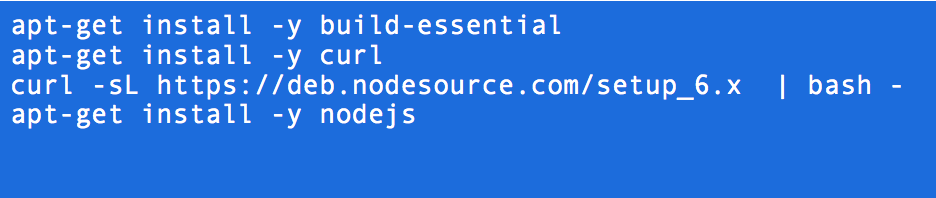
\includegraphics[width=120mm]{node.png}
    \end{figure}
    \subsubsection{Java JDK}
    \begin{figure}[H]
    \centering
    
\includegraphics[width=120mm]{java.png}
    \end{figure}
  \subsection{System Requirements}
  The only system requirement is that you must be logged in as root user on Debian 8.
\section{User Guide}
  \subsection{Home Page}
  After completing the installation phase, the application will be ready to use. The landing page will look like
  fig:1.
  \begin{figure}[H]
  \centering
  
\includegraphics[width=120mm]{home.png}
  \caption{Spikes Home Page}
  \end{figure}
  Welcome to SPIKES! From the homepage you can choose from three tabs at the top of the page; ‘Analysis’, ‘Static Data File’ or ‘Live Stream’.
  The ‘Static Data File’ tab is where to go when you have uploaded a file in the ‘Analysis’ tab, here it will show you all the anomalies in the data.
  The ‘Live Stream’ tab is identical to the ‘Static Data File’ but is for live stream data instead.
  \subsection{Analysis tab}
  The Analysis tab is the starting point of the app, here you can upload either a static data file or enter an input stream source, along with stopping and starting the analysis.
  In order to select the other two tabs, analysis will have to have been initiated on this page.
  \begin{figure}[H]
  \centering
  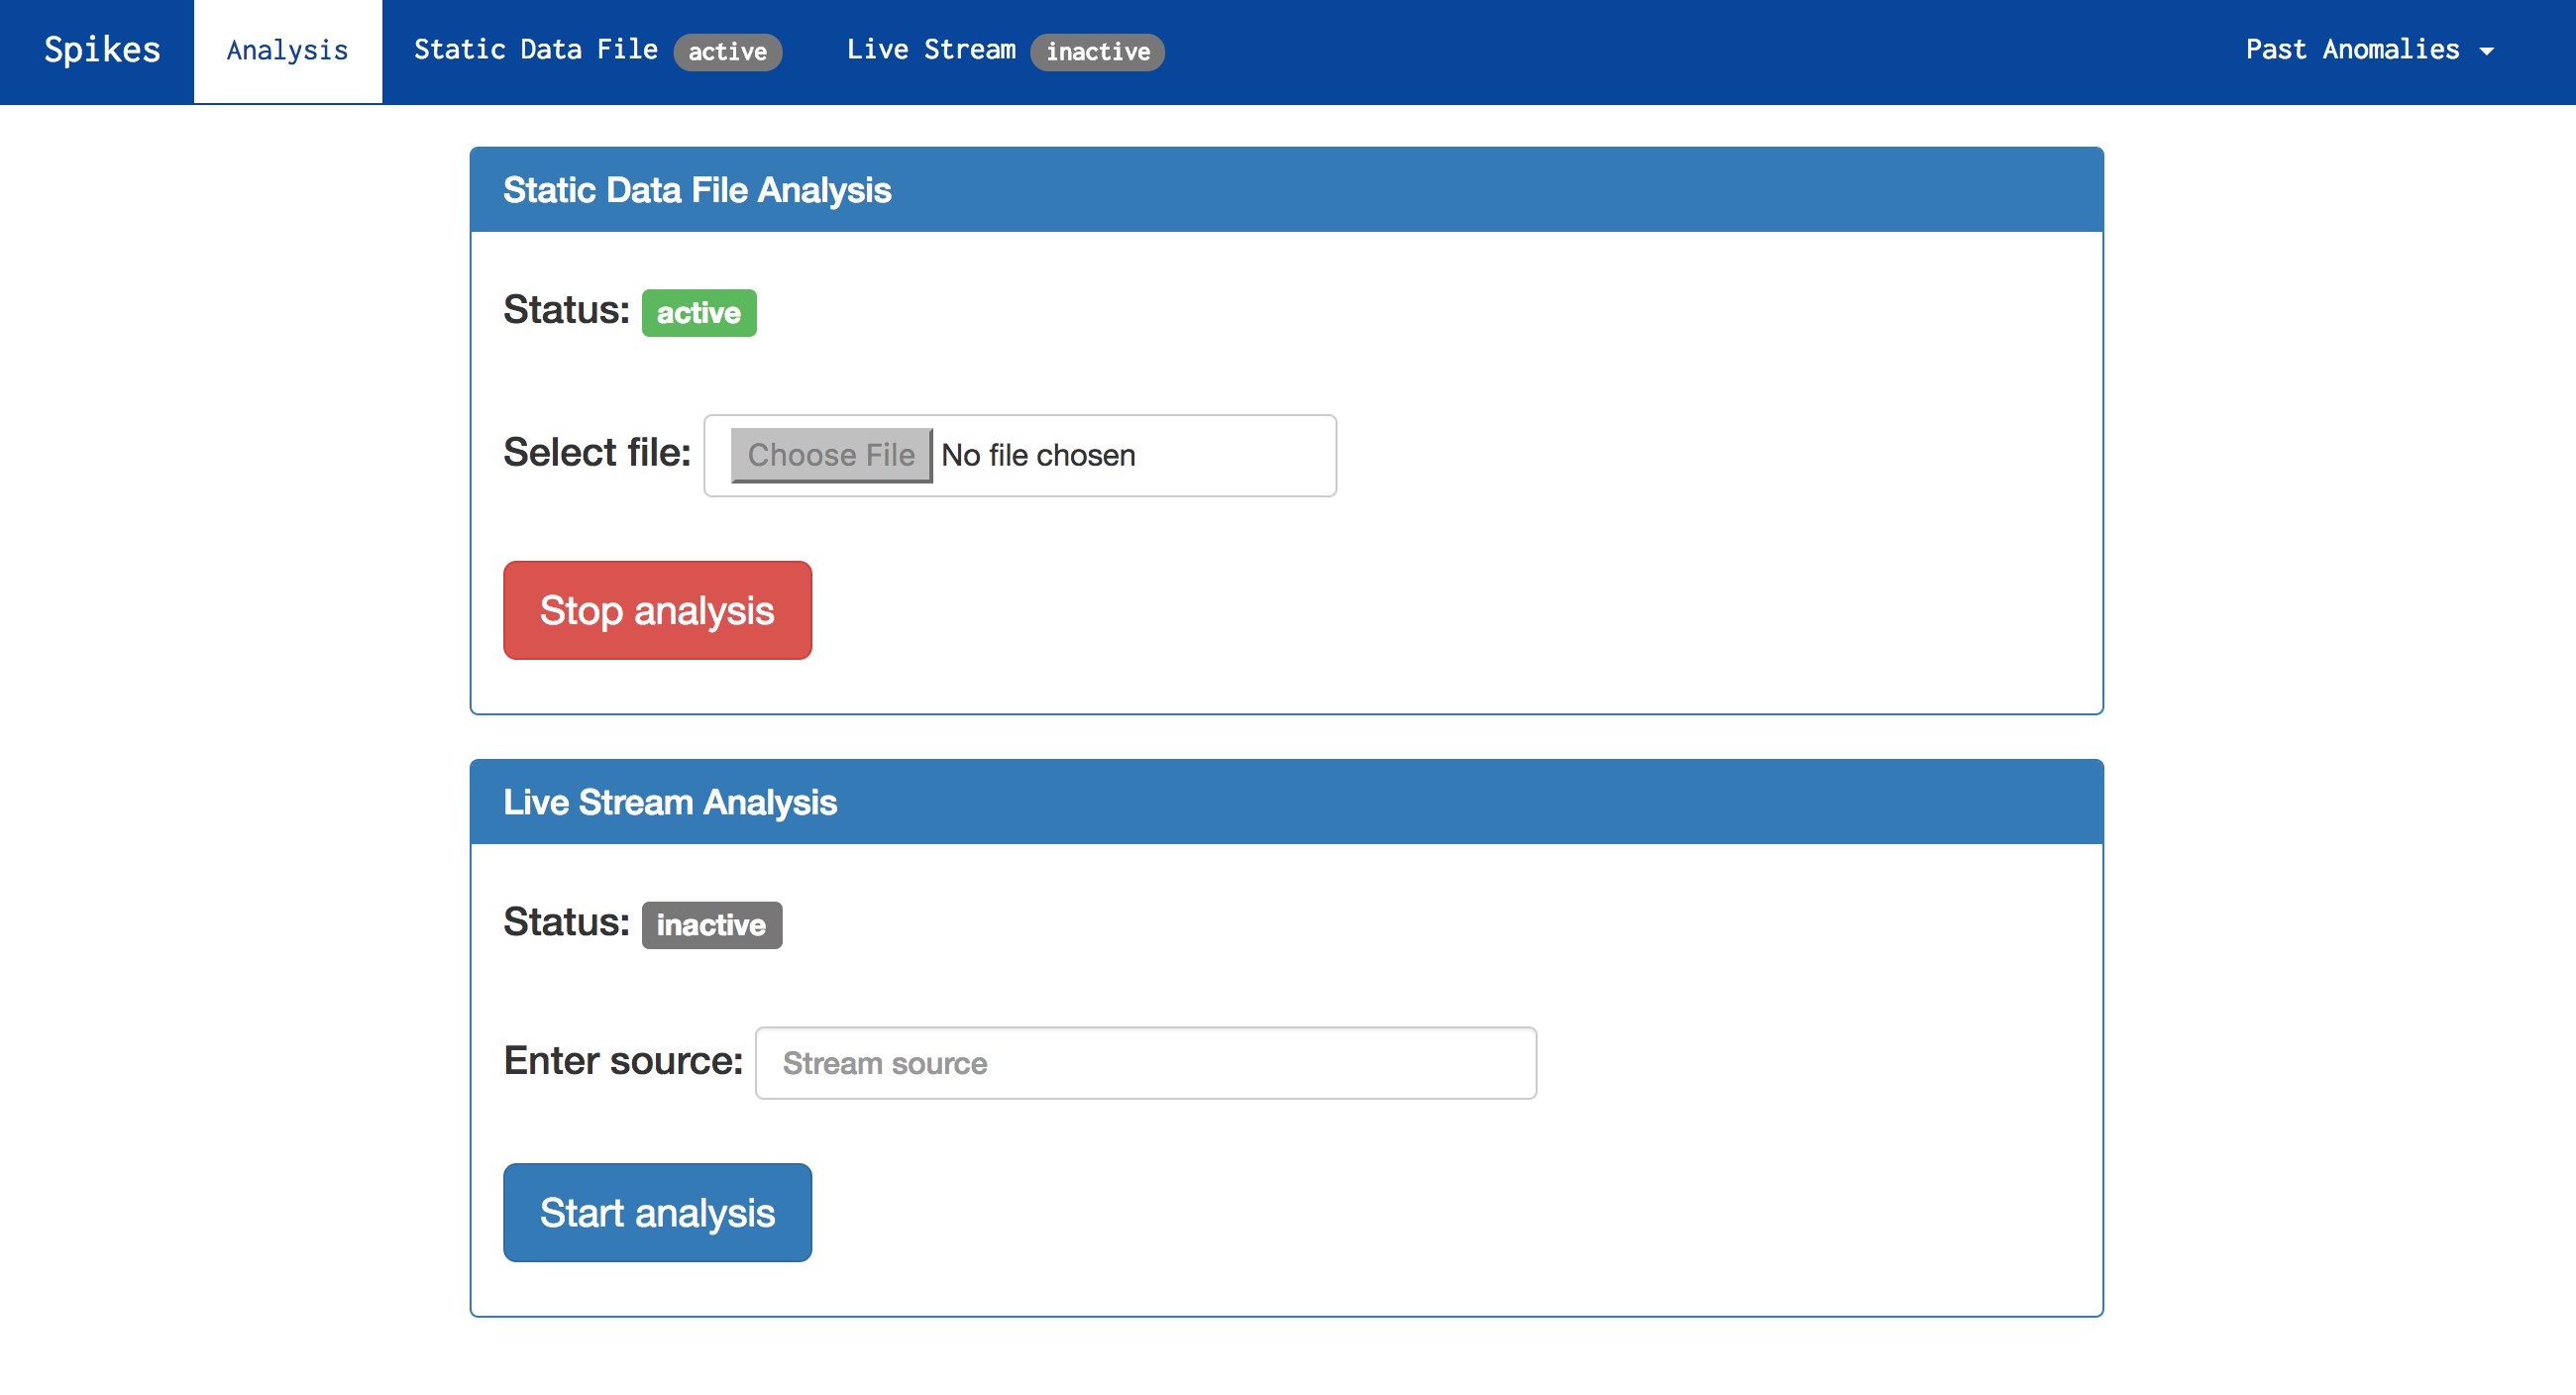
\includegraphics[width=120mm]{analysisTab.png}
  \caption{Analysis Tab}
  \end{figure}
  It consists of two controllers, one for static historical data and the other for a live stream data.
  Each controller has two options; upload and start analysis. There are no file size restrictions when uploading given sufficient hard disk storage.
  By commencing analysis, it will alert you that analysis is active, you will then be allowed to navigate to the corresponding tab.
  \subsection{Live Stream tab/Historical Data tab}
  When analysis is started, anomalies will start to be detected and generated in the respective tab, each anomaly that is detected will appear as an alert box on the page.
  Alerts contain only crucial data such as; Type of Anomaly, Symbol, Date and a drop down arrow that leads to more specific data.
  Volume spikes and price manipulation alerts will have a drill down button that generates a graph surronding displaying the suspicous data.
\section{Research}
  After the analysis and design of the project, our software development team had developed a stronger idea
  of the technologies that would be used to design the system. This section further expands on the decisions and
  research that was made after the first deliverable that allowed us to finalise our choice of technologies.
  \subsection{Front-end}
  We decided as a whole group quite early that the whole application would be web-based rather than a desktop app. This would
  increase the accessibility of the application being cross-browser compatible and mobile friendly. If the client integrated a sufficient
  security system, the system could be accessed from anywhere with a secure internet connection.\newline
  The \textbf{AngularJS} framework was used to build the frontend as planned. We considered other JavaScript frameworks,
  such as \textbf{React}, however we felt that AngularJS was the better choice being a full-fledged MVC (Model-View-Controller) framework.
  As our system is a single page application (SPA) that will update dynamically, AngularJS became a natural choice for our developers.
  \newline
  After this decision was made between the Project Manager and Developers, our front-end developers took the initiative to intensively learn AngularJS using a multitude online resources.
  For example, Codecademy a programming teaching platform was used to learn AngularJS basics, whilst AngularJS Community pages were used to further expand their knowledge.
  \subsubsection{JavaScript Graph Library}
  Deciding on a suitable JavaScript Graph Library was crucial for this project as data visualisation was one of our major non-functional requirements.
  After extensive research we decided to use the \textbf{PlotlyJS} library for the following reasons:
  \begin{itemize}
    \itemsep0em
    \item It generates responsive graphs that are able to scale dynamically on different platforms e.g. desktops, tablets
    \item PlotlyJS is known for use in financial analytics and supports a variety of graphs e.g. candlestick, boxplots
    \item Uses WebGL technology for graph rendering with a speed that surpasses many competitors
    \item Provides the option to export the rendered graphs as PNG files for further inspection if needed
    \item Allows the zooming into of graphs, allowing the user to further inspect specific areas of the graph
  \end{itemize}
  \subsection{Back-end}
    \subsubsection{Server-Side}
    Node.js was used as our interface between the frontend and the Java backend using the Express framework.
    This decision was made by the Back-end developers built on their exisiting skills with JavaScript. Node is extremely fast,
    compiling JavaScript code directly into machine code using Google's V8 engine, this means when facing large volumes of data
    the system will stay responsive due to the way Node handles concurrency. The modules and templates written in node can be easily
    reused throughout the serverside, thus reducing the size of our application and chance of bugs occuring.
    \newline
    Other popular server-side-scripts were considered such as Django and Ruby on Rails but given the unfamiliarity and time
    constraints, we discarded them because they did not fully utilise the current skills of the developers.
    \subsubsection{Database}
    Deciding whether to store stock data into a MySQL database became a frequently debated topic throughout the development of the application.
    If the system integrated a database ; storing the input stream into the database for a reasonable time period, it would allow us to
    select relevant data at will and improve the chance of the system finding potential perpetrators of any malicious anomalies.
    \newline
    Despite this, if the system relied on the database too heavily, a performance bottleneck would occur. Thus, making our system slower and less responsive.
    Our developer's countermeasure to this was to cache the data within Java's abstract data structures and storing data for a certain amount
    of time until the oldest data would be useful in further algorithmic calculations.
    \newline
    Once the Back-end developers had come to a decision. It was then agreed between the whole group to run the system without a database, thus avoiding
    any bottlenecks and creating a multi-threaded application with minimal lag.
\section{Design}
  \subsection{User Interface}
         The main focus of the user interface was to provide a view so simplistic and natural that the client would not even consider using the provided manual. After sending the mock UI design
         to the client and received positive feedback, the front-end team decided to use the mockups as a guidline.\newline
         The color scheme of the user interface primarily uses a familiar but refreshing blue because it provides a contrast that does not strain the eye and draws the visual attention of the user.
         The font size used throughout the interface follows the universal usability principles such that the more important the information is the larger the font. Therefore, the larger text is scanned
         and smaller text is read more carefully. Also, the separation of functions onto individual tabs, prevents the user from being overwhelmed with information.
         \begin{figure}[H]
         \centering
         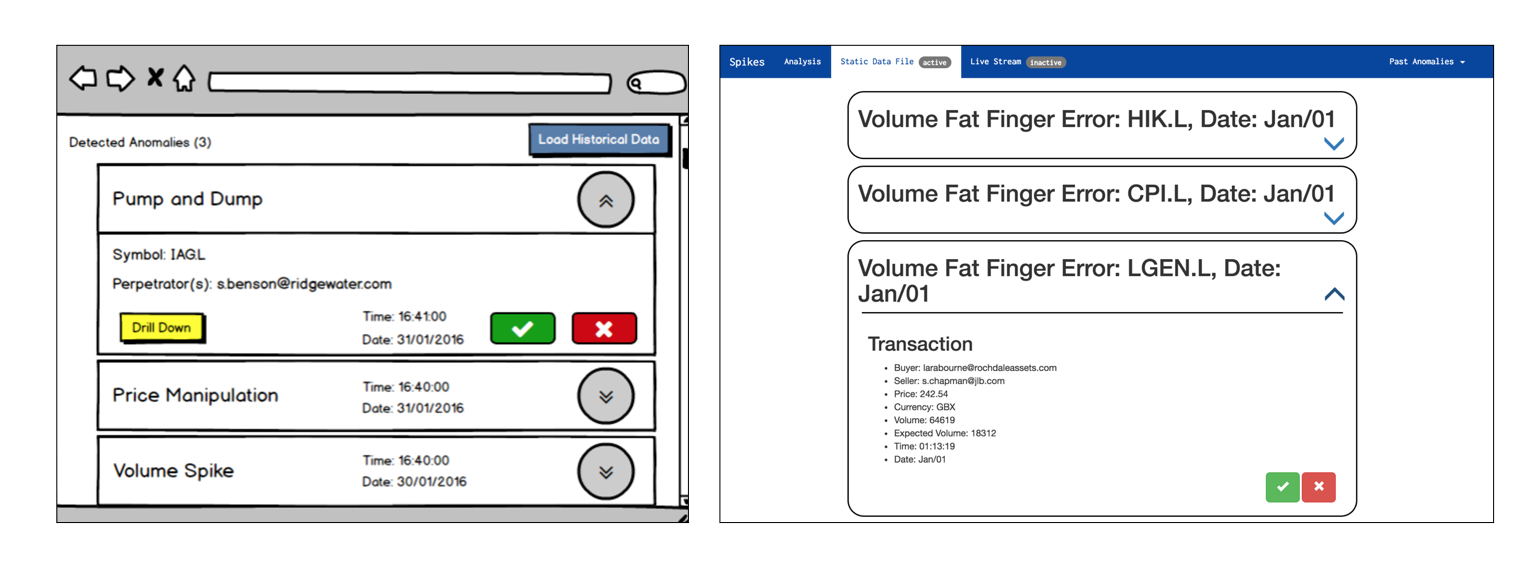
\includegraphics[width=170mm]{ui1.png}
         \caption{Evolution of user interface}
         \end{figure}
  \subsection{Pseudocode}
    This section explores the type of algorithms that we used to analyse the input stream of data for anomalies.
    \subsubsection{Pump \& Dump}
    Arguably, Pump \& Dump was the most challenging type of price manipulation that we attempted to detect.
    After researching the characteristics of a Pump \& Dump, our team concluded the following about Pump \& Dump:
    \begin{itemize}
      \itemsep0em
      \item A large batch of cancellation orders will occur before the dumping of stocks by a person or group (\textbf{Undetectable with current data set})
      \item A steady increase of stock value from the average, when the pumping state begins (\textbf{Detectable})
      \item A sudden drop in stock value when the dumping of stocks occur (\textbf{Detectable})
    \end{itemize}
    \begin{figure}[H]
    \centering
    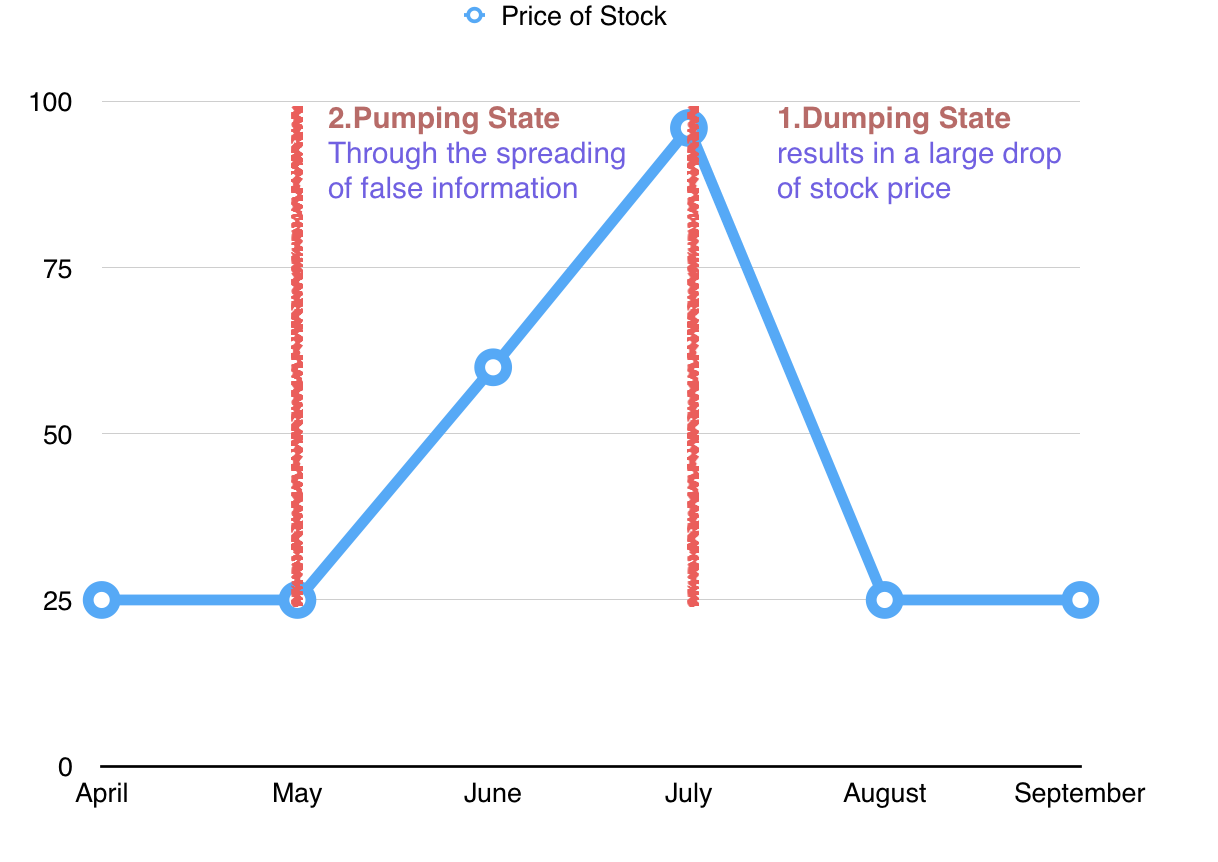
\includegraphics[width=100mm]{PumpDumpGraph.png}
    \caption{Pump \& Dump Example}
    \end{figure}
    By identifying the traits of a Pump \& Dump, we were able to build the above model in fig:4.
    We found it more intuitive to design an algorithm that would first detect a dumping state, then look back
    on historical data to detect whether a pumping state had occured before the drop in stock value. Below in fig:5 is the
    pseudocode that would later be transformed into Java code.
    \begin{figure}[H]
    \centering
    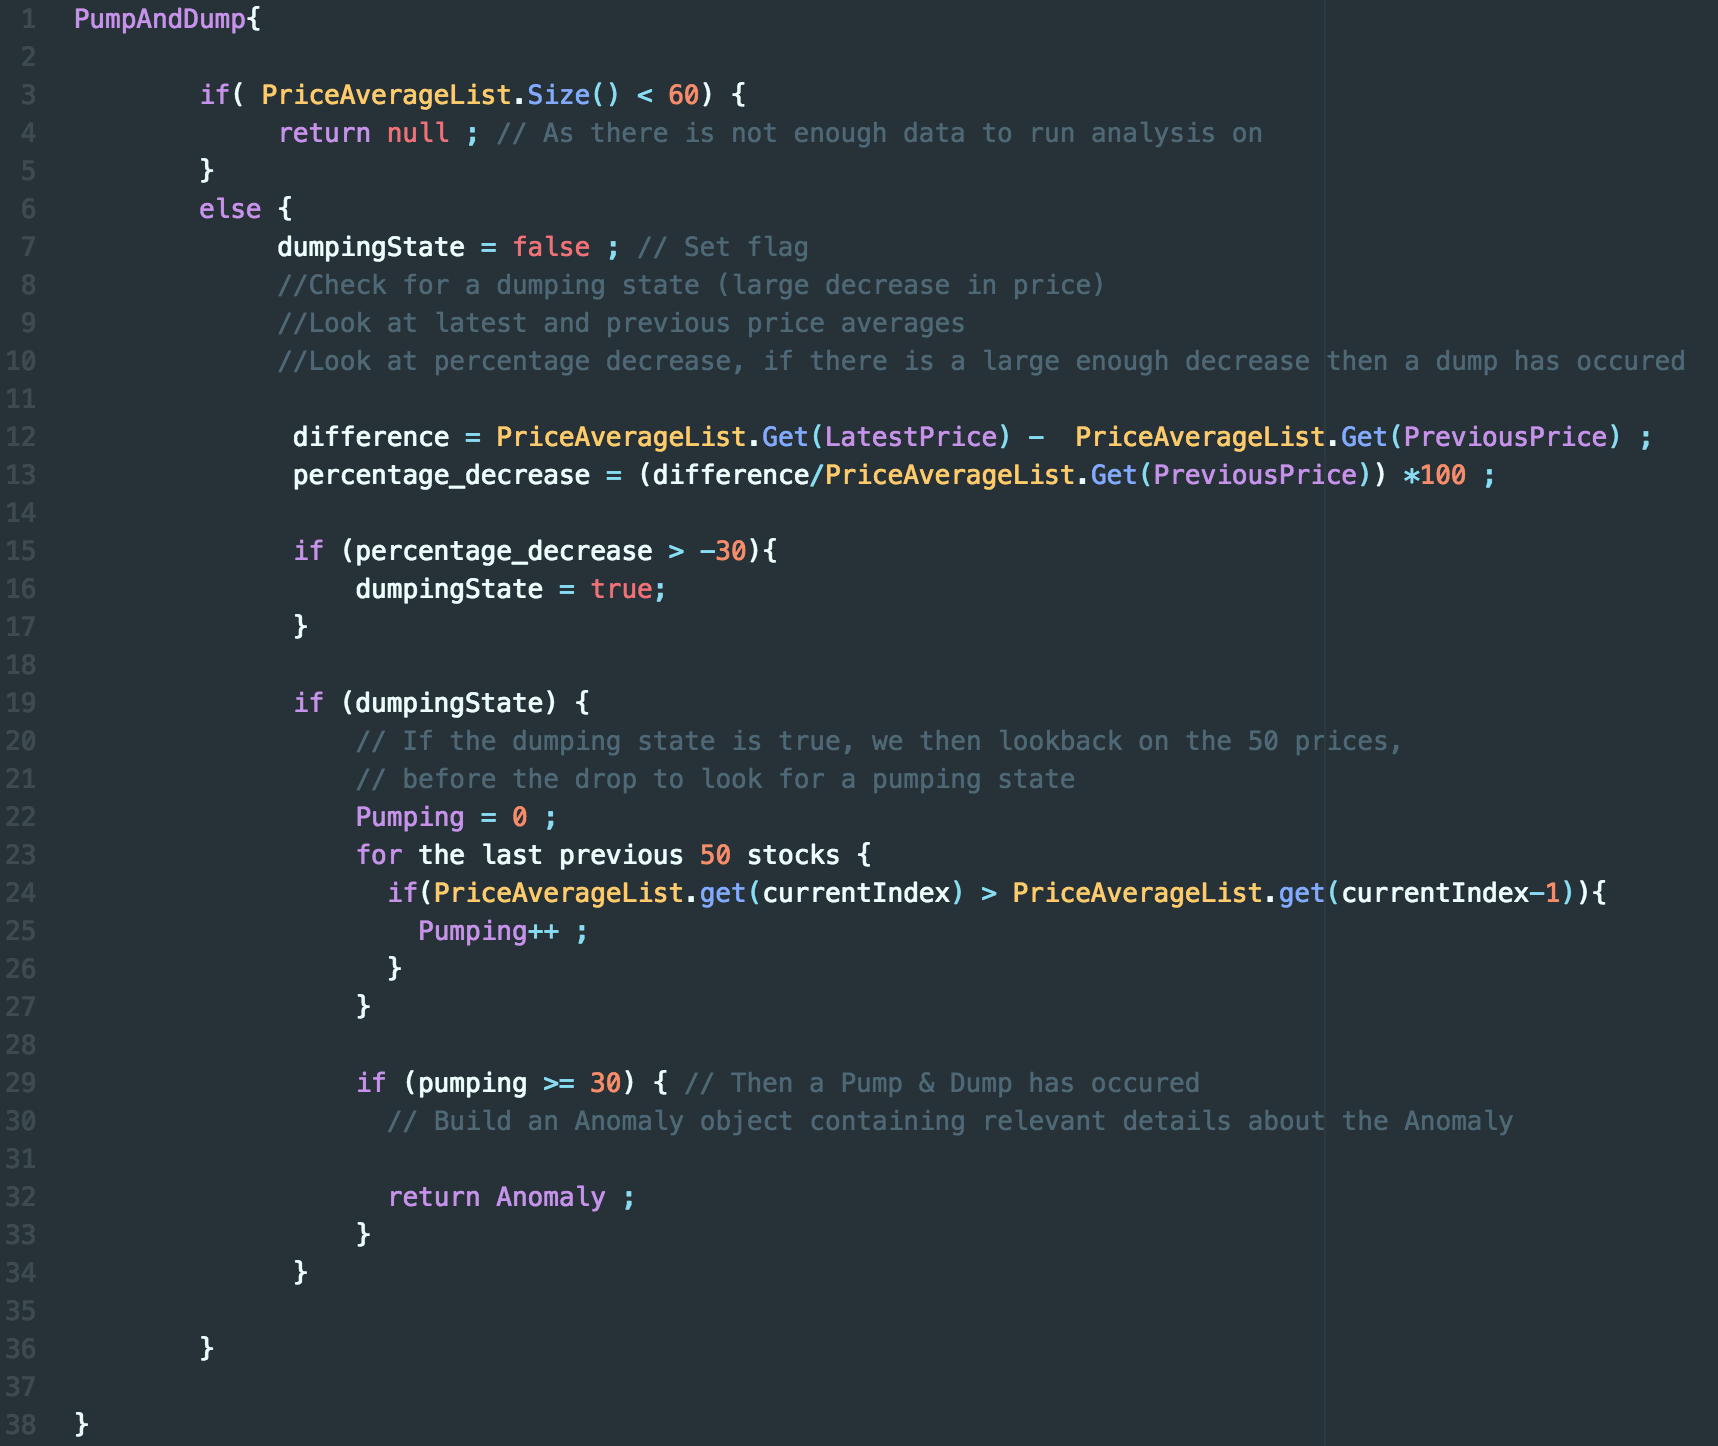
\includegraphics[width=150mm]{PDpseudo.png}
    \caption{Pump \& Dump Pseudocode}
    \end{figure}
    \subsubsection{Volume Spike}
    To detect volume spikes, the algorithm keeps track of the amount of stocks bought within a certain time interval and calculates a volume moving average (VMA) that will be used as a comparison for the consequent interval. Therefore, if the total stock
    volume in a period greatly surpasses that of the previous VMA by a user-controlled threshold. The program will flag a volume spike, as seen below in fig:6. The threshold level would then adjust it's sensitivity to spikes depending on the user's feedback.
    \begin{figure}[H]
    \centering
    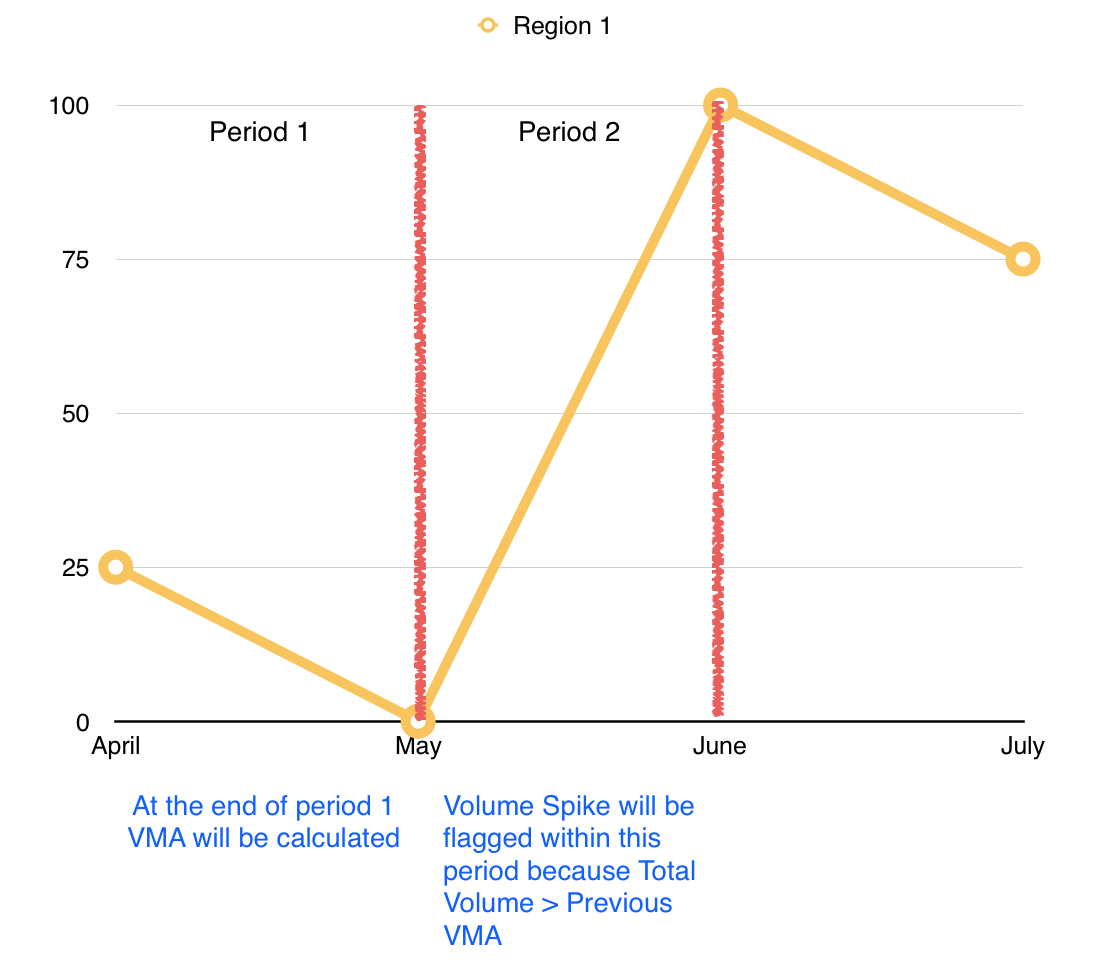
\includegraphics[width=80mm]{VSGraph.png}
    \caption{Volume Spike Example}
    \end{figure}
    \begin{figure}[H]
    \centering
    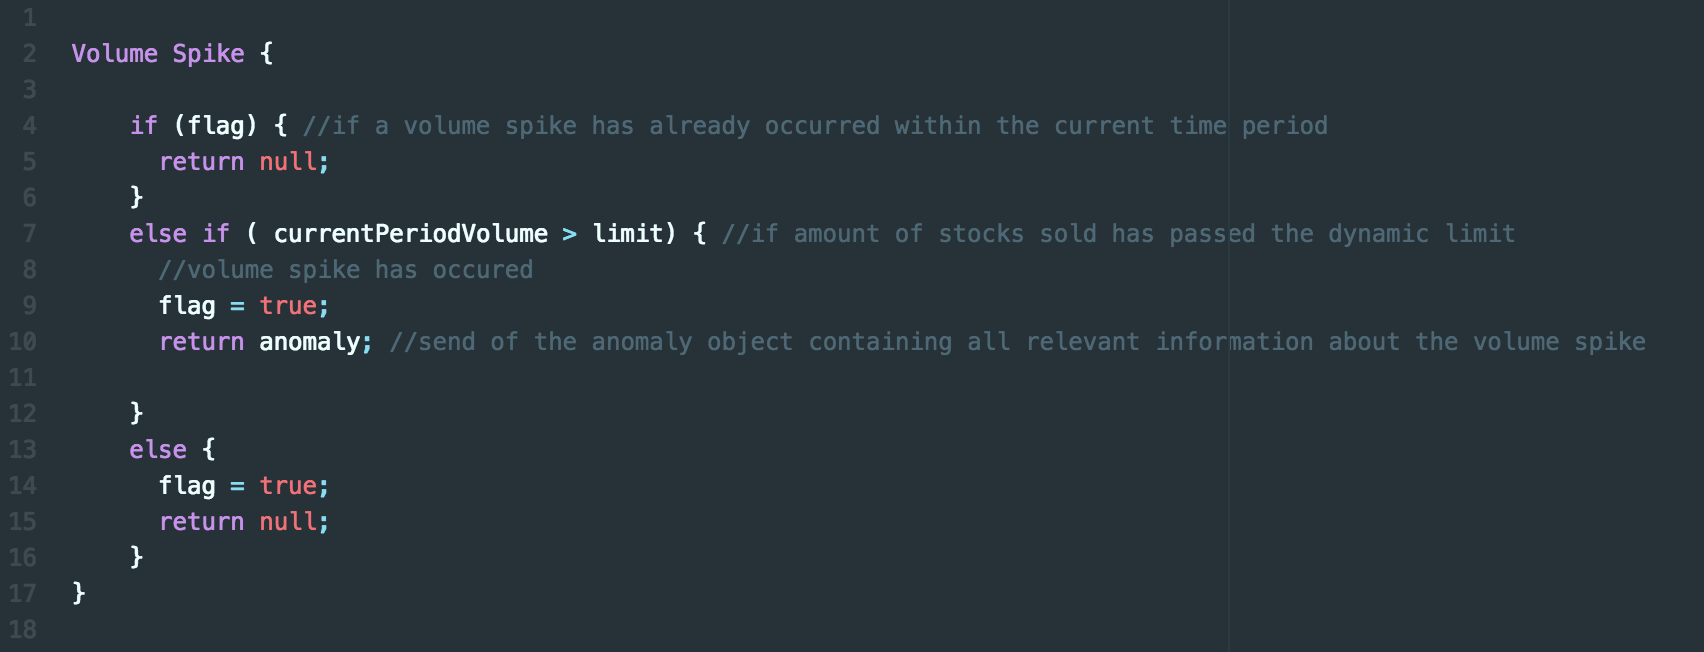
\includegraphics[width=150mm]{VSpseudo.png}
    \caption{Volume Spike Pseudocode}
    \end{figure}
    \subsubsection{Fat Finger Errors}
    When detecting fat finger errors we decided to separate the error into two types:
    \begin{itemize}
      \itemsep0em
      \item Fat Finger \textbf{Price Error}, which will detect fat finger errors related to the price of a stock transaction
      \item Fat Finger \textbf{Volume Error}, which will detect fat finger errors related to the size of a stock transaction
    \end{itemize}
    This is because it is possible for the Price or Size of a transaction to be extremely large compared to the average due to a typing fat finger error.
    The algorithm we developed to detect fat finger errors, uses orders of magnitude to determine whether the price or volume is extremely larger or smallerf than the average (in factors of ten).
    \begin{figure}[H]
      \centering
      \begin{minipage}{0.4\textwidth}
        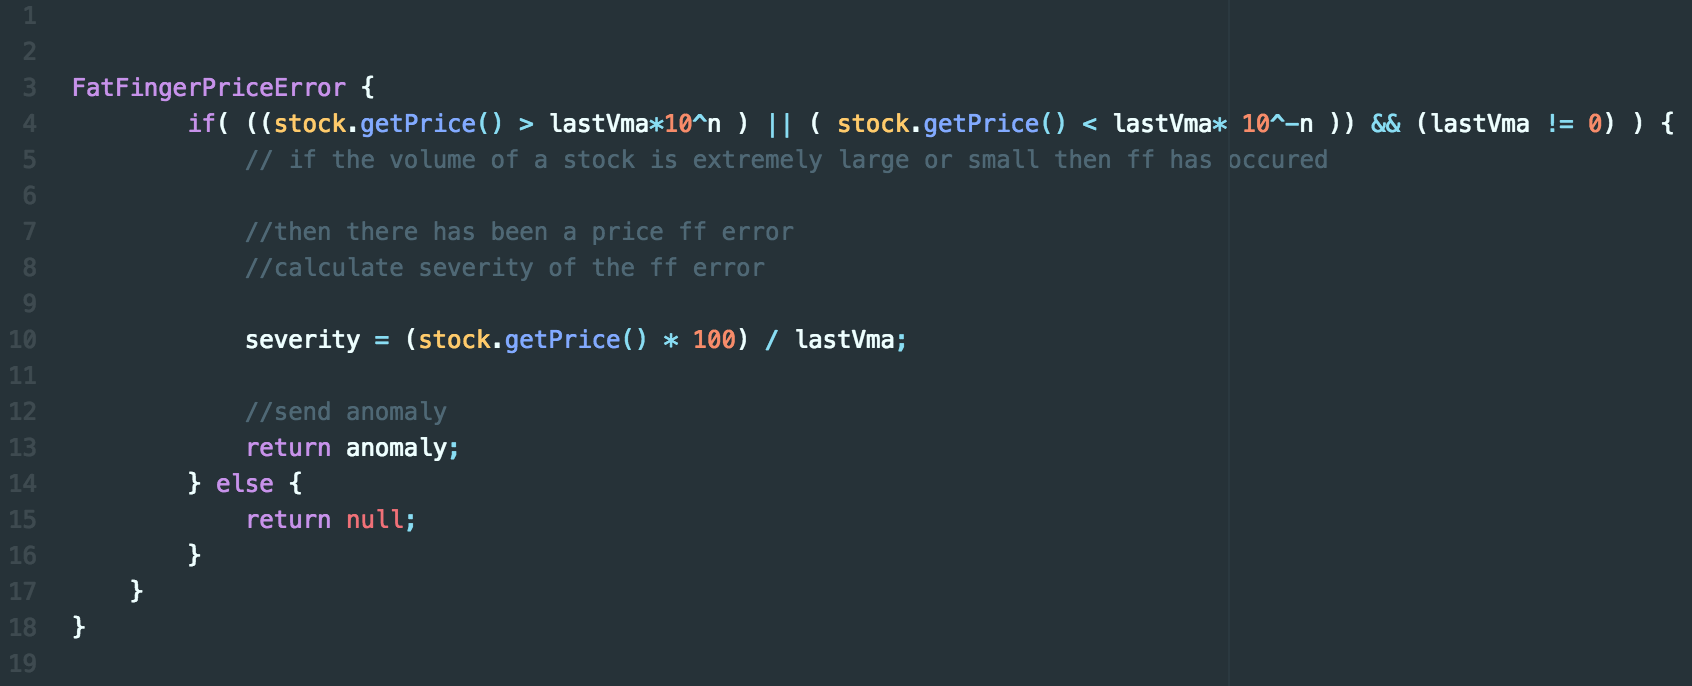
\includegraphics[width=\textwidth]{FFprice.png}
        \caption{FF Price Pseudocode}
      \end{minipage}
      \begin{minipage}{0.4\textwidth}
        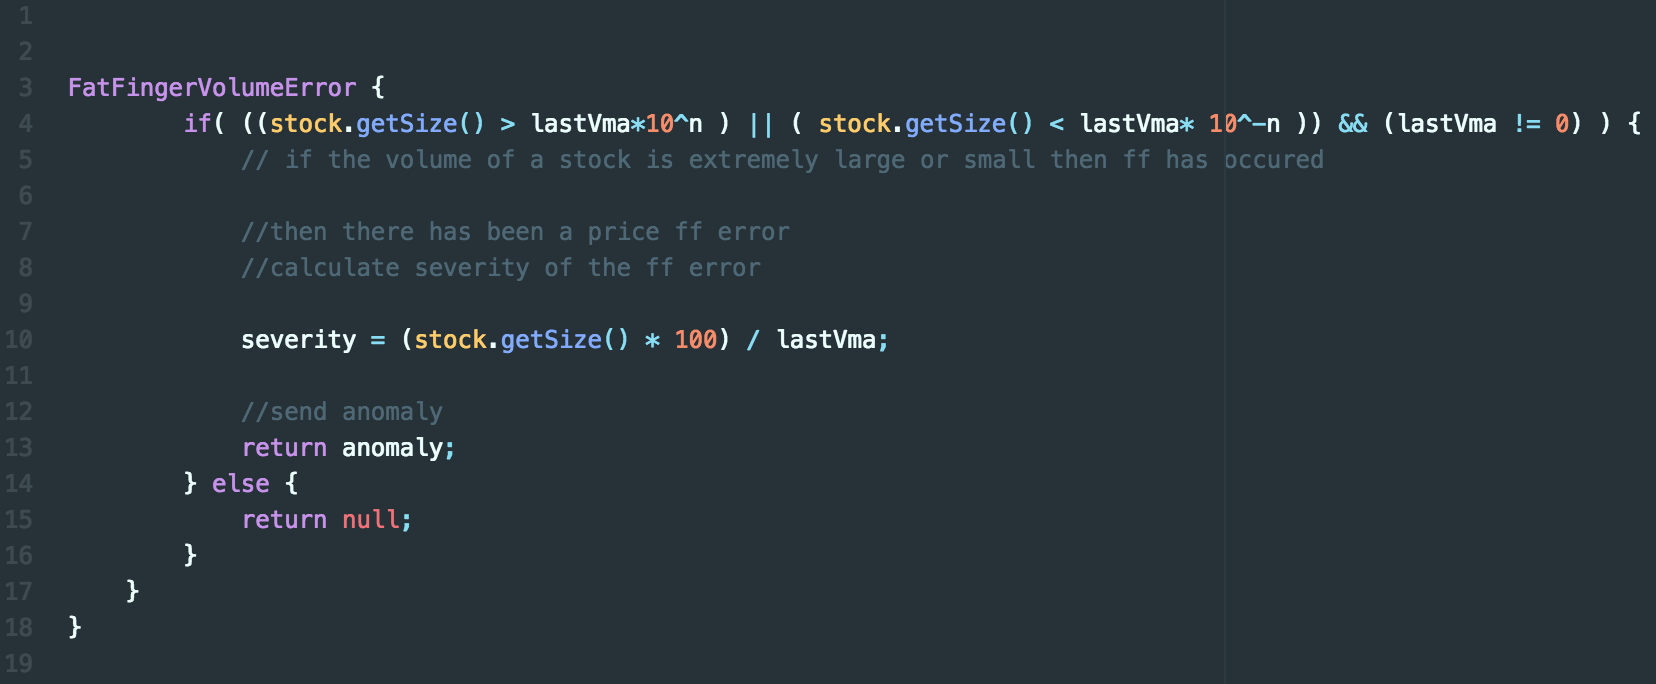
\includegraphics[width=\textwidth]{FFvolume.png}
        \caption{FF Volume Pseudocode}
      \end{minipage}
    \end{figure}
\section{Implementation}
  \subsection{Frontend}
  The front end parsing and displaying of anomaly data is predominantly performed using AngularJS, PlotlyJS and Socket.io.
  The CSS framework Bootstrapa was used to design the UI and make it responsive on various platforms.
  All data sent by the back end server follows a strict interface to guarantee the proper generation of alerts on the user’s screen. An AngularJS module stores a buffer of anomaly data packages.
  Once these anomalies arrive, they are picked up from the module buffer by an AngularJS controller. This controller identifies anomaly types and uses a predefined HTML template to generate the website elements.
  The templates use AngularJS expressions as placeholders for specific anomaly data (e.g. stock symbols, time) as well as functions which call different front end components, such as graph charting functions.
  Graphs are generated with plotly using an array of Y-axis Values and the JS will calculate the X-axis values by converting the initial epoch value, and using an interval length to calculate the rest.
  \subsection{Backend}
  The back end consists entirely of a java program, which is formed of several objects, for extraction, analysis and sending JSON to the front end.
  The program is run through a central control object, which takes arguments to decide data source(file or stream) and then starts the relevant extraction thread. As the thread is running the controller checks the queue, and for each object in the queue the symbol is checked, then the relevant checks occur on that symbol via an array of check objects stored in a hash table(by symbol).
  Each array contains 4 check objects: one for volume spikes, two for fat fingers and one for pump \& dump. All check objects implement the ICheck interface, which ensures that other check objects can be made and used with the system in future.
  When a check object detects an anomaly, it returns an anomaly object specific to the anomaly (an abstract class allows for generic methods to be used on this, again allowing for future additions) these anomaly objects are then picked up by the controller parsed into JSON and sent through a socket to the front end. Unfortunately, due to several issues being encountered with multiple generic libraries for JSON conversion, the conversion has been hardcoded.
  However due to the modular approach taken, this issue is minor and should a library be made to work it could be easily implemented without altering the body of the program in any way.
    \subsubsection{Parsing}
    All data parsing took place in java using the input stream reader, and file reader libraries to extract data from stream and file respectively.
    The stream uses an infinite loop to repeatedly check the stream for new data packets, each of which is then sent to a separate method called stockBuilder.
    Similarly the file is read through line by line until the end of the document, with each being sent to stockBuilder.
    In stockBuilder the data is separated by commas and parsed into a stock object. The constituents of the stock object are passed to the object as is, with the exception of the numbers (which were converted to their numerical form) and the date, which thanks to the SimpleDateFormat library, is converted to a long in the form milliseconds since linux epoch.
    In both cases the resulting stock object is added to the end of a queue. Both stream and file extraction are run on threads, allowing analysis to run concurrently with extraction. All interaction between the threads and the program take place through the queue, which is synchronised at all points of use to ensure thread safety.
\section{Sprint Cycles}
  This section gives an overview on what each sprint cycle accomplished and how our system evolved using an agile approach.
  \subsection{Sprint Cycle 1}
  \begin{figure}[H]
  \centering
  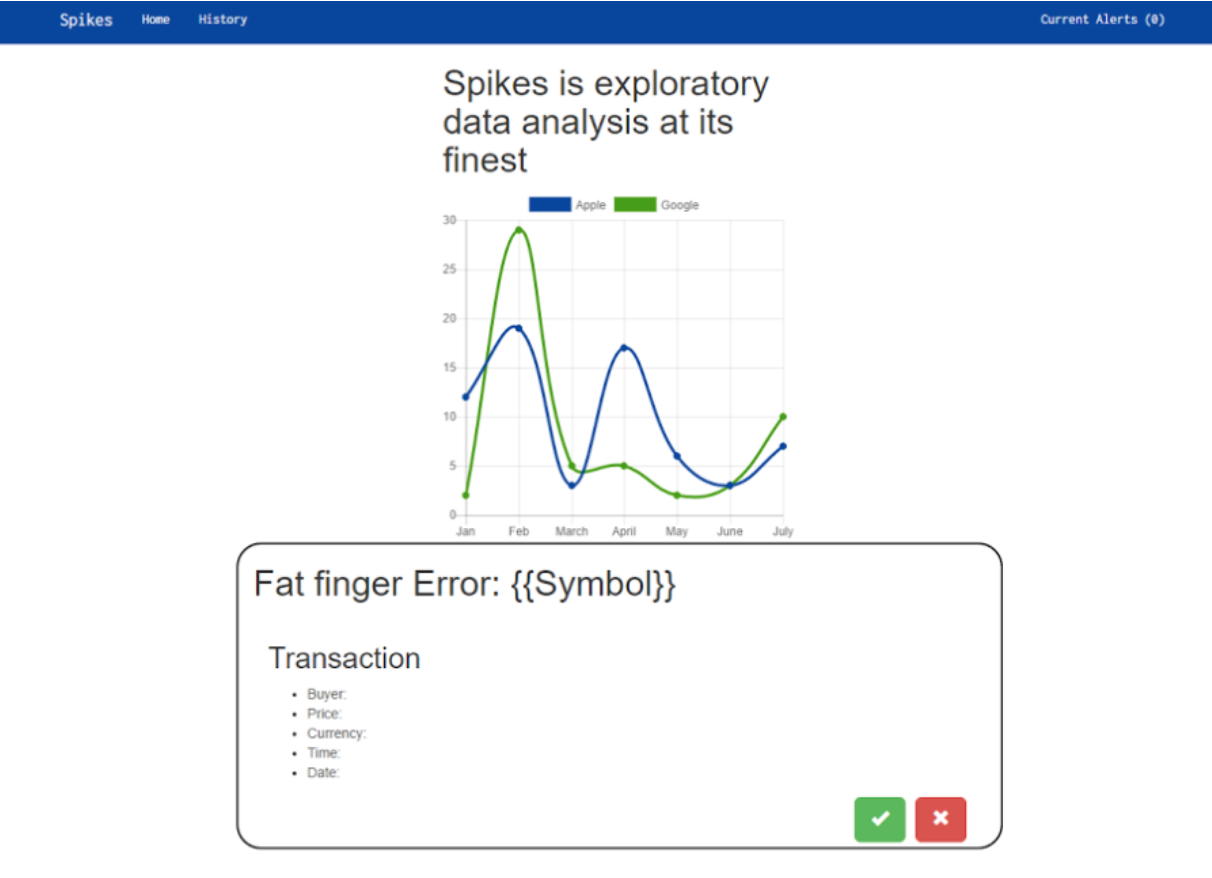
\includegraphics[width=80mm]{sprint1.png}
  \caption{Initial UI skeleton}
  \end{figure}
  The first sprint cycle consisted of our back-end team designing the various algorithms while the front-end team worked on the UI skeleton simultaneously.
  We wanted to get the skeleton of the UI implemented as soon as possible, so that there was more available time for refinement.
  Initially, we had two pages; ‘Home’ and ‘History’. The ‘Home’ page would show all the anomalies and the ‘History’ tab would have past anomalies that have since been removed from the ‘Home’ page.
  The graph at the top of the page was created with Chart.js charting library and was used to give the team an idea what an example graph would look like.
  The anomalies would appear within the structures below the graph, where the user could either accept or reject the anomaly.
  \subsection{Sprint Cycle 2}
  \begin{figure}[H]
  \centering
  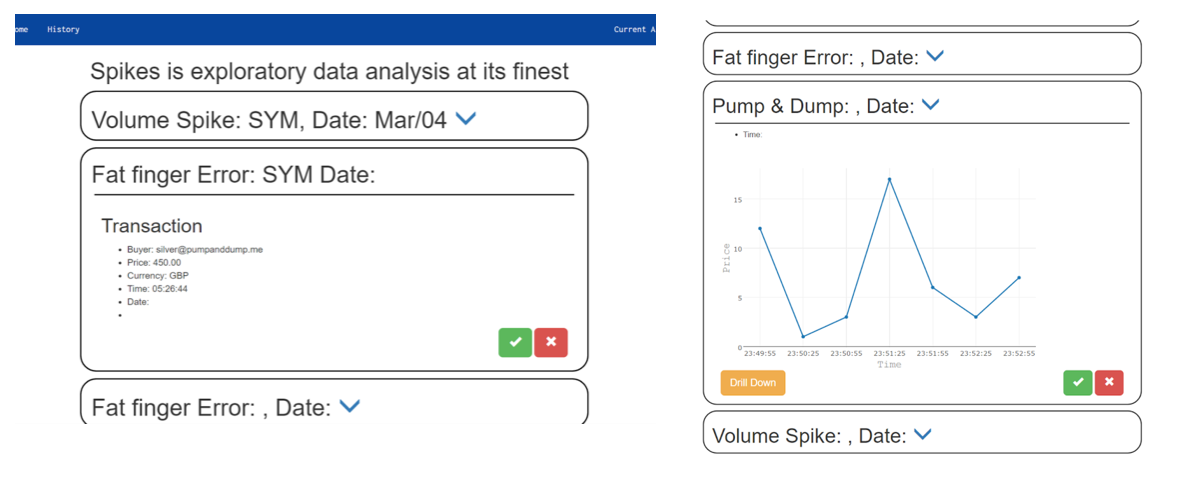
\includegraphics[width=100mm]{sprint2.png}
  \caption{Development of alert boxes}
  \end{figure}
  In the second sprint cycle. We implemented the drop down arrow on the alert boxes so that design resembled the mockup more. We decided that the type of anomaly, symbol and date were the most important details regarding an anomaly, so these details were left outside of the drop down.
  It was also decided in the sprint cycle review meeting that Chart.js was insufficient to show the necessary data, instead Plotly.JS was used in its place as it provides much more features and an extensive range of graph types.
  The ‘Drill Down’ button was implemented for volume spike and pump \& dump, when clicked it would render a graph which would provide a better analysis of the anomaly.
  \subsection{Sprint Cycle 3}
  \begin{figure}[H]
  \centering
  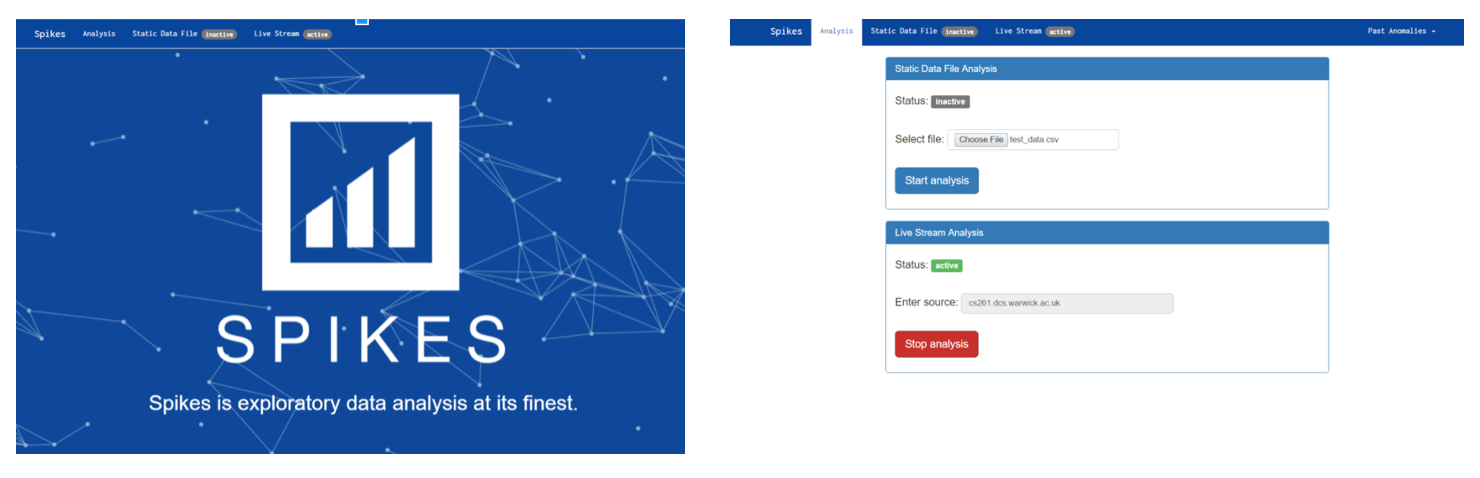
\includegraphics[width=100mm]{sprint3.png}
  \caption{Introduction of Spikes 2.0}
  \end{figure}
  In the third sprint cycle, a major update to the UI occurred. A new homepage and logo were designed.
  We added three new tabs; ‘Analysis’, ‘Static Data File’ and ‘Live Stream’.
  We also implemented the pseudocode for volume spike, the implementation required various adjustments
  as errors were realised throughout testing and eventually overcome.
  At this point, we were only able to test the algorithm with mock data collected in the Java back-end.
  \subsection{Sprint Cycle 4}
  \begin{figure}[H]
  \centering
  \includegraphics[width=80mm]{sprint4.png}
  \caption{Volume spike detection fully functional}
  \end{figure}
  In the fourth sprint cycle we implemented the pseudocode for fat finger errors, initially it used simple bounds to detect an error,
  however after some research  we decided to use orders of magnitude, however this wasn’t working how we imagined it to do so.
  A realisation occurred in this sprint review meeting ; that two types of fat finger could possibly occur (Price/Volume).
  Our target for the next sprint cycle was to implement a fully-functional algorithm to detect Pump \& Dump, with the system fully connected.
  \subsection{Sprint Cycle 5}
  \begin{figure}[H]
  \centering
  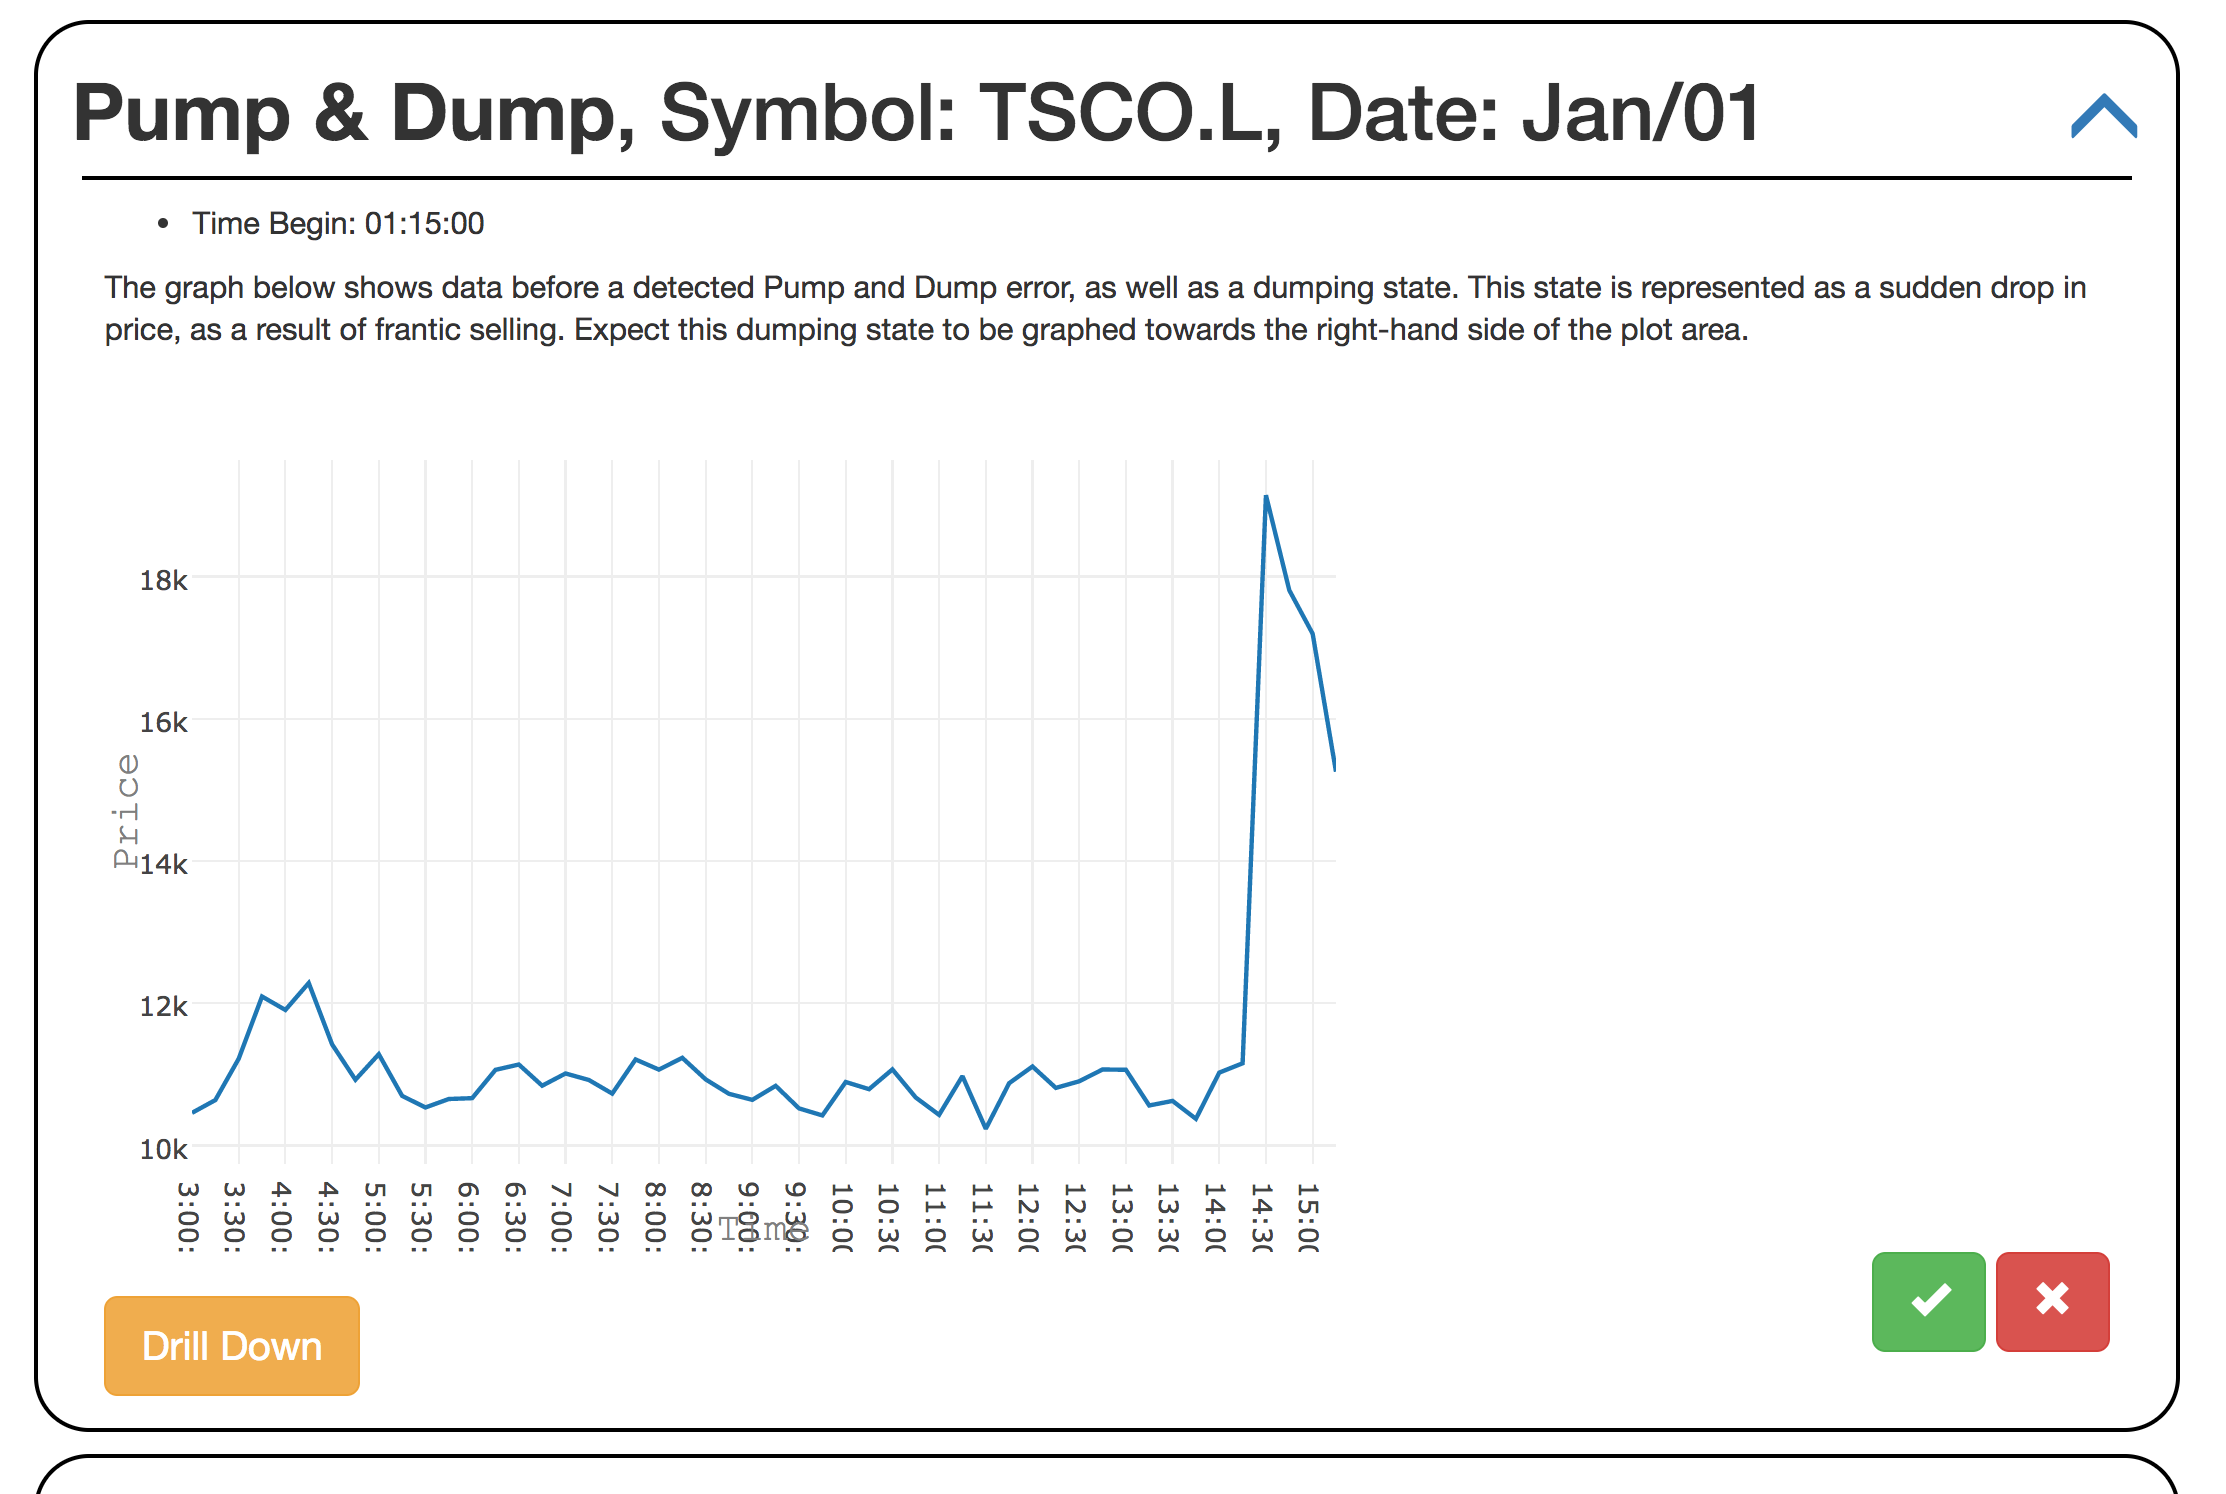
\includegraphics[width=80mm]{sprint5.png}
  \caption{Pump \& Dump detection fully functional}
  \end{figure}
  In the final sprint cycle, we implemented the algorithm for Pump \& Dump.
  This was most challenging for our team and although we had created the pseudocode in an earlier week we realised that this was not the optimal solution.
  After some discussion as a team we decided upon a solution that could work, however implementation proved to be just as difficult.
  After tweaking the sensitivity we managed to get the pump \& dump detection to a state that all team members deemed suitable.
\section{Testing}
  Throughout the development process, new test data was fabricated by each developer during the implementation of each feature.
  Therefore, we are confident that the majority of faults were uncovered due to the variety of test cases that the overall solution was subjected to.
  \subsection{Unit Testing}
  During the implementation of our solution, each feature was tested as it was developed to ensure correct functioning before integration.
  This strategy allowed the developers to carry out unit testing specifically designed for each minor component, as they were implemented, removing any bugs early on.
  The result of ongoing testing was a deep understanding of these individual components which helped the development team better understand and fix later issues.
    \subsubsection{Front-end Testing}
    In the interest of providing a responsive and interactive user interface (UI), the front-end HTML and CSS development team systematically tackled each activity
    that the user may have had to carry out using the application through the UI. Any errors related to interface feedback and the interaction between the user and the system were fixed at this stage.
    This provided a medium through which the development team could interact with the system and test further features.
    \newline
    Regarding the proper processing of flagged anomalies by the AngularJS front-end, the UI alert generation was tested using fabricated JSON packets of anomaly data.
    Once these packets were received, the testers observed the generated UI elements for any discrepancies and made any necessary modifications.
    During this process, an interface template to be used between the front-end and back-end was decided upon by the entire development team to provide consistency across software components.
    \begin{figure}[H]
    \centering
    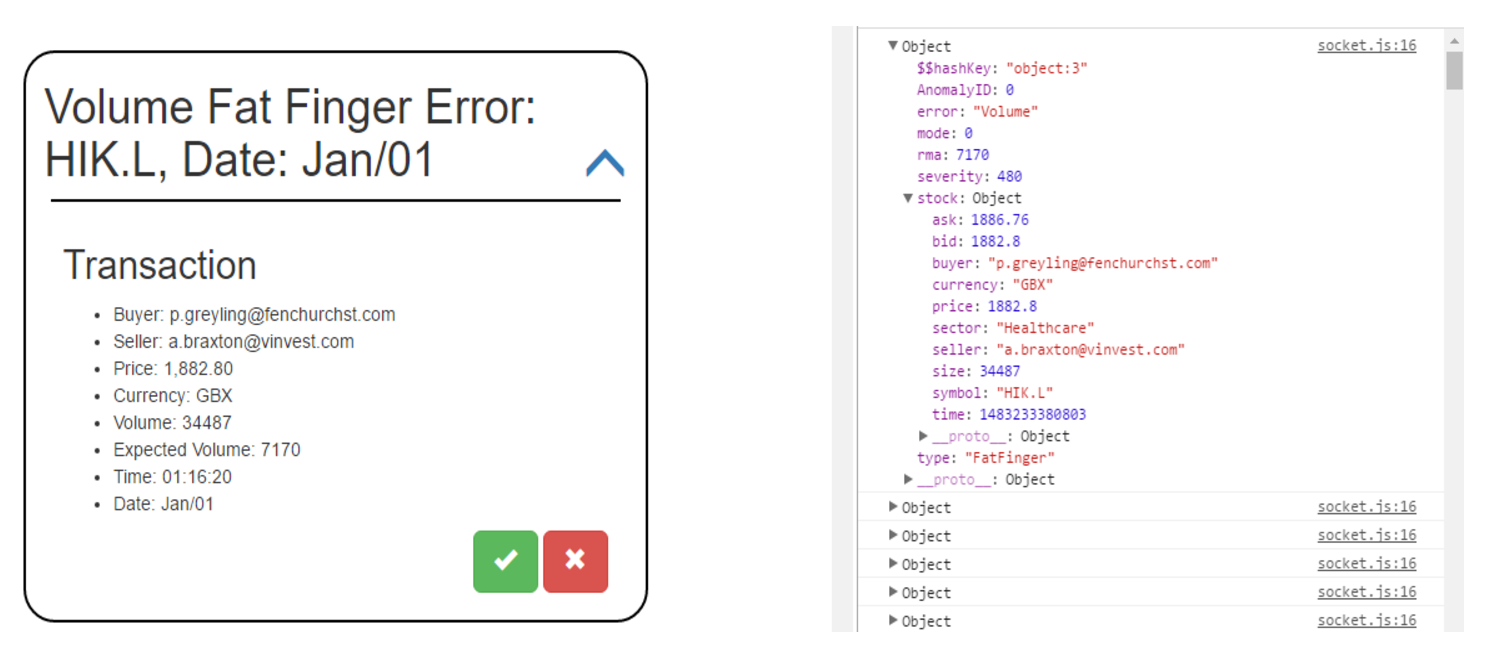
\includegraphics[width=130mm]{test1.png}
    \caption{Testing of alert generation with mock data}
    \end{figure}
    \subsubsection{Back-end Testing}
    All Java implementations of the analysis algorithms were subjected to intensive tests using the historical data provided, the live trade stream and fabricated trade data.
    The purpose of these tests was to verify that the algorithms were calculating reasonable values and flagging anomalous results correctly.
    Console reports (image num), printed during implementation of algorithms, were used to reveal the data processing done by the back-end.
    \begin{figure}[H]
    \centering
    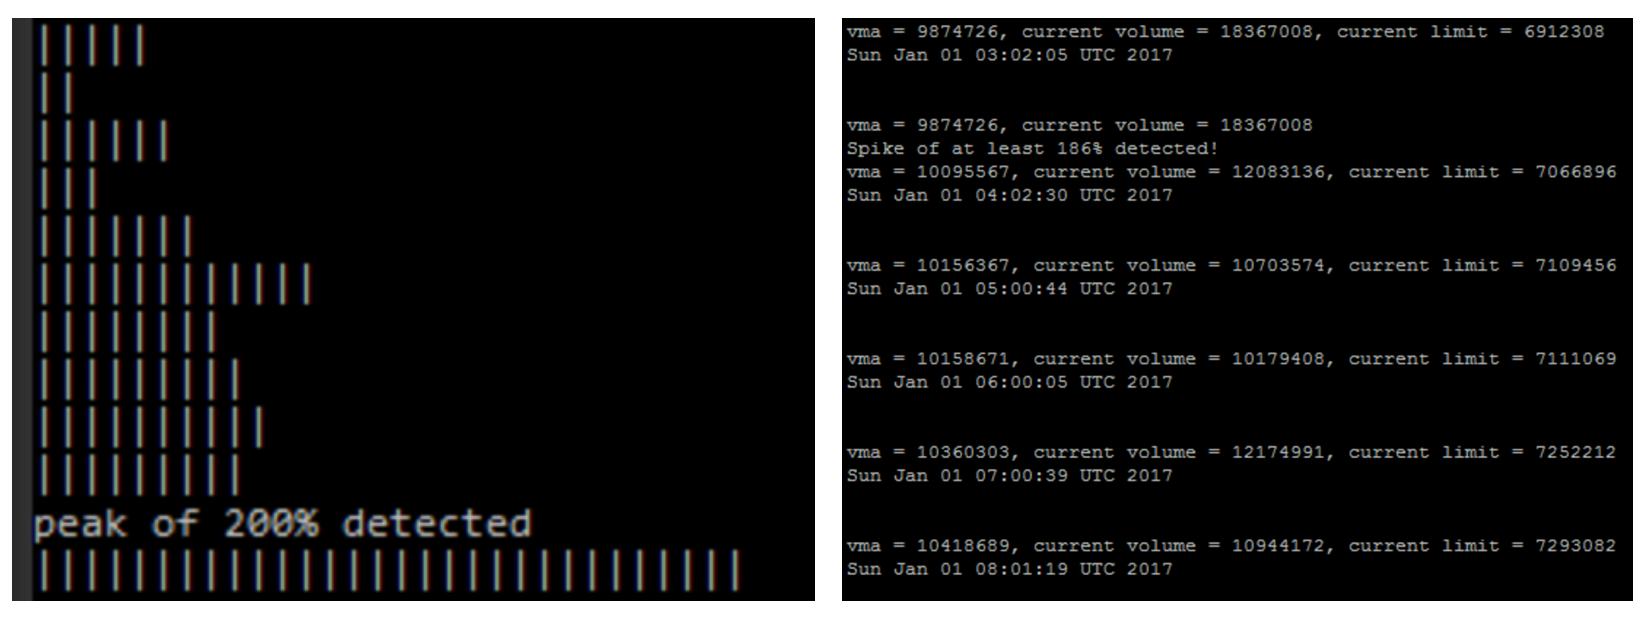
\includegraphics[width=130mm]{backtest.png}
    \caption{Testing of Java analysis algorithms}
    \end{figure}
    In addition, output data to be passed to the front-end was displayed to ensure that all interfaces established between developers were taken into consideration.
	  Finally, all anomaly data being displayed had to be buffered by the NodeJS server before it was sent to the front-end. The development team observed data flowing into and out of the NodeJS server,
    and checked data stored by the server against expected formats and values. Removal of errors at this stage provided confidence in the transmission of data from the back-end processing to the front-end client view.
    \subsection{Integration Testing}
    Once each feature was completed, tested and debugged, it was integrated into the overall solution. Firstly, the node server was connected the Java back-end analyser using sockets and after this connection was fully tested.
    Secondly, the Node was connected to the Angular through socket.io, providing mock packets before the entire came together. Upon integration, tests were constructed and executed on the resulting, enhanced application.
    At this point, issues such as parsing errors were discovered by the front-end developers due to the mulititude of different templates generated by the angular and resolved before they could affect later versions.
    In this way, the team was able to ensure that any errors which appeared after the integration of a new component were strictly related to the component.
    This lead to easier debugging during each development iteration.
    \subsection{System Testing}
    Working versions of the application were tested using Black-Box Testing: fabricated data which contained patterns of real anomalies was fed into the software and resulting errors were checked for consistency with expectations. Additionally, working system versions were tested against the provided trade data files.
    The output of these tests was reviewed and checked against relevant parts of the input data to confirm that the anomalies were indeed relevant and the data displayed was correct.
  	In addition to verifying correct detection of anomalies and transmission of data to the user, robustness and reliability were ensured by passing erroneous trade data to the analysis tool.
    This data included trades with missing fields or wrong types of data. The back-end development team set checks in place such that, even in such cases the system functioned correctly and the erroneous data did not affect later results.
    \subsection{User Acceptance Testing}
    In order to provide an application which was in line with expectations from the client, all features implemented were based on the initial Requirements Analysis, and Design and Implementation reports. According to the feedback received, our listed system requirements represented what is expected from the end product.
    Furthermore, the User Interface provided is based on the sketches delivered to Deutsche Bank, which received a positive reaction.
    \subsection{Non-Functional Testing}
    The application was also tested to satisfy non-functional qualities. The system performance was measured in terms of time taken to carry out processing and to display anomalies.
    This was done in the final sprint cycle. During an early period of development in which the system used SQL databases to store a large amount of data for eventual retrieval and analysis, we identified that database access tasks took a very long time.
    As a consequence, all other tasks would have to wait, and the entire system was noticeably slower. To mitigate this issue, all database storage was made redundant and the database was completely removed from the process.
  	Secondly, usability of the interface was tested by trials with users chosen randomly. The layout proved to be intuitive and easy to use, even for an inexperienced test subject. Moreover, all clickable areas were designed to be large and easy to use, and the colour scheme is suitable for colour blind users.

\section{Project Management}
  \subsection{Overview}
  Overall the team worked well together. A project manager was assigned early (Sylvester) who assigned everyone else’s role based on their skillset and prior knowledge. No one felt like they were given the wrong role and we were all comfortable with the tasks we had been given.
  Group meetings were held twice per week to catch up on each other’s progress and collaborate when necessary, and communication in between meetings was maintained over online services such as Slack and Facebook Messenger. Program code and documentation was kept synchronised between the development teams using GitHub and Google Drive. This level of collaboration was crucial, so that progress could be tracked to ensure deadlines were met and so the team could give and receive help from each other when needed.
  All of the team members collaborated in the writing of the deliverable documents, contributing to the sections relevant to their roles in the project.
  \begin{figure}[H]
  \centering
  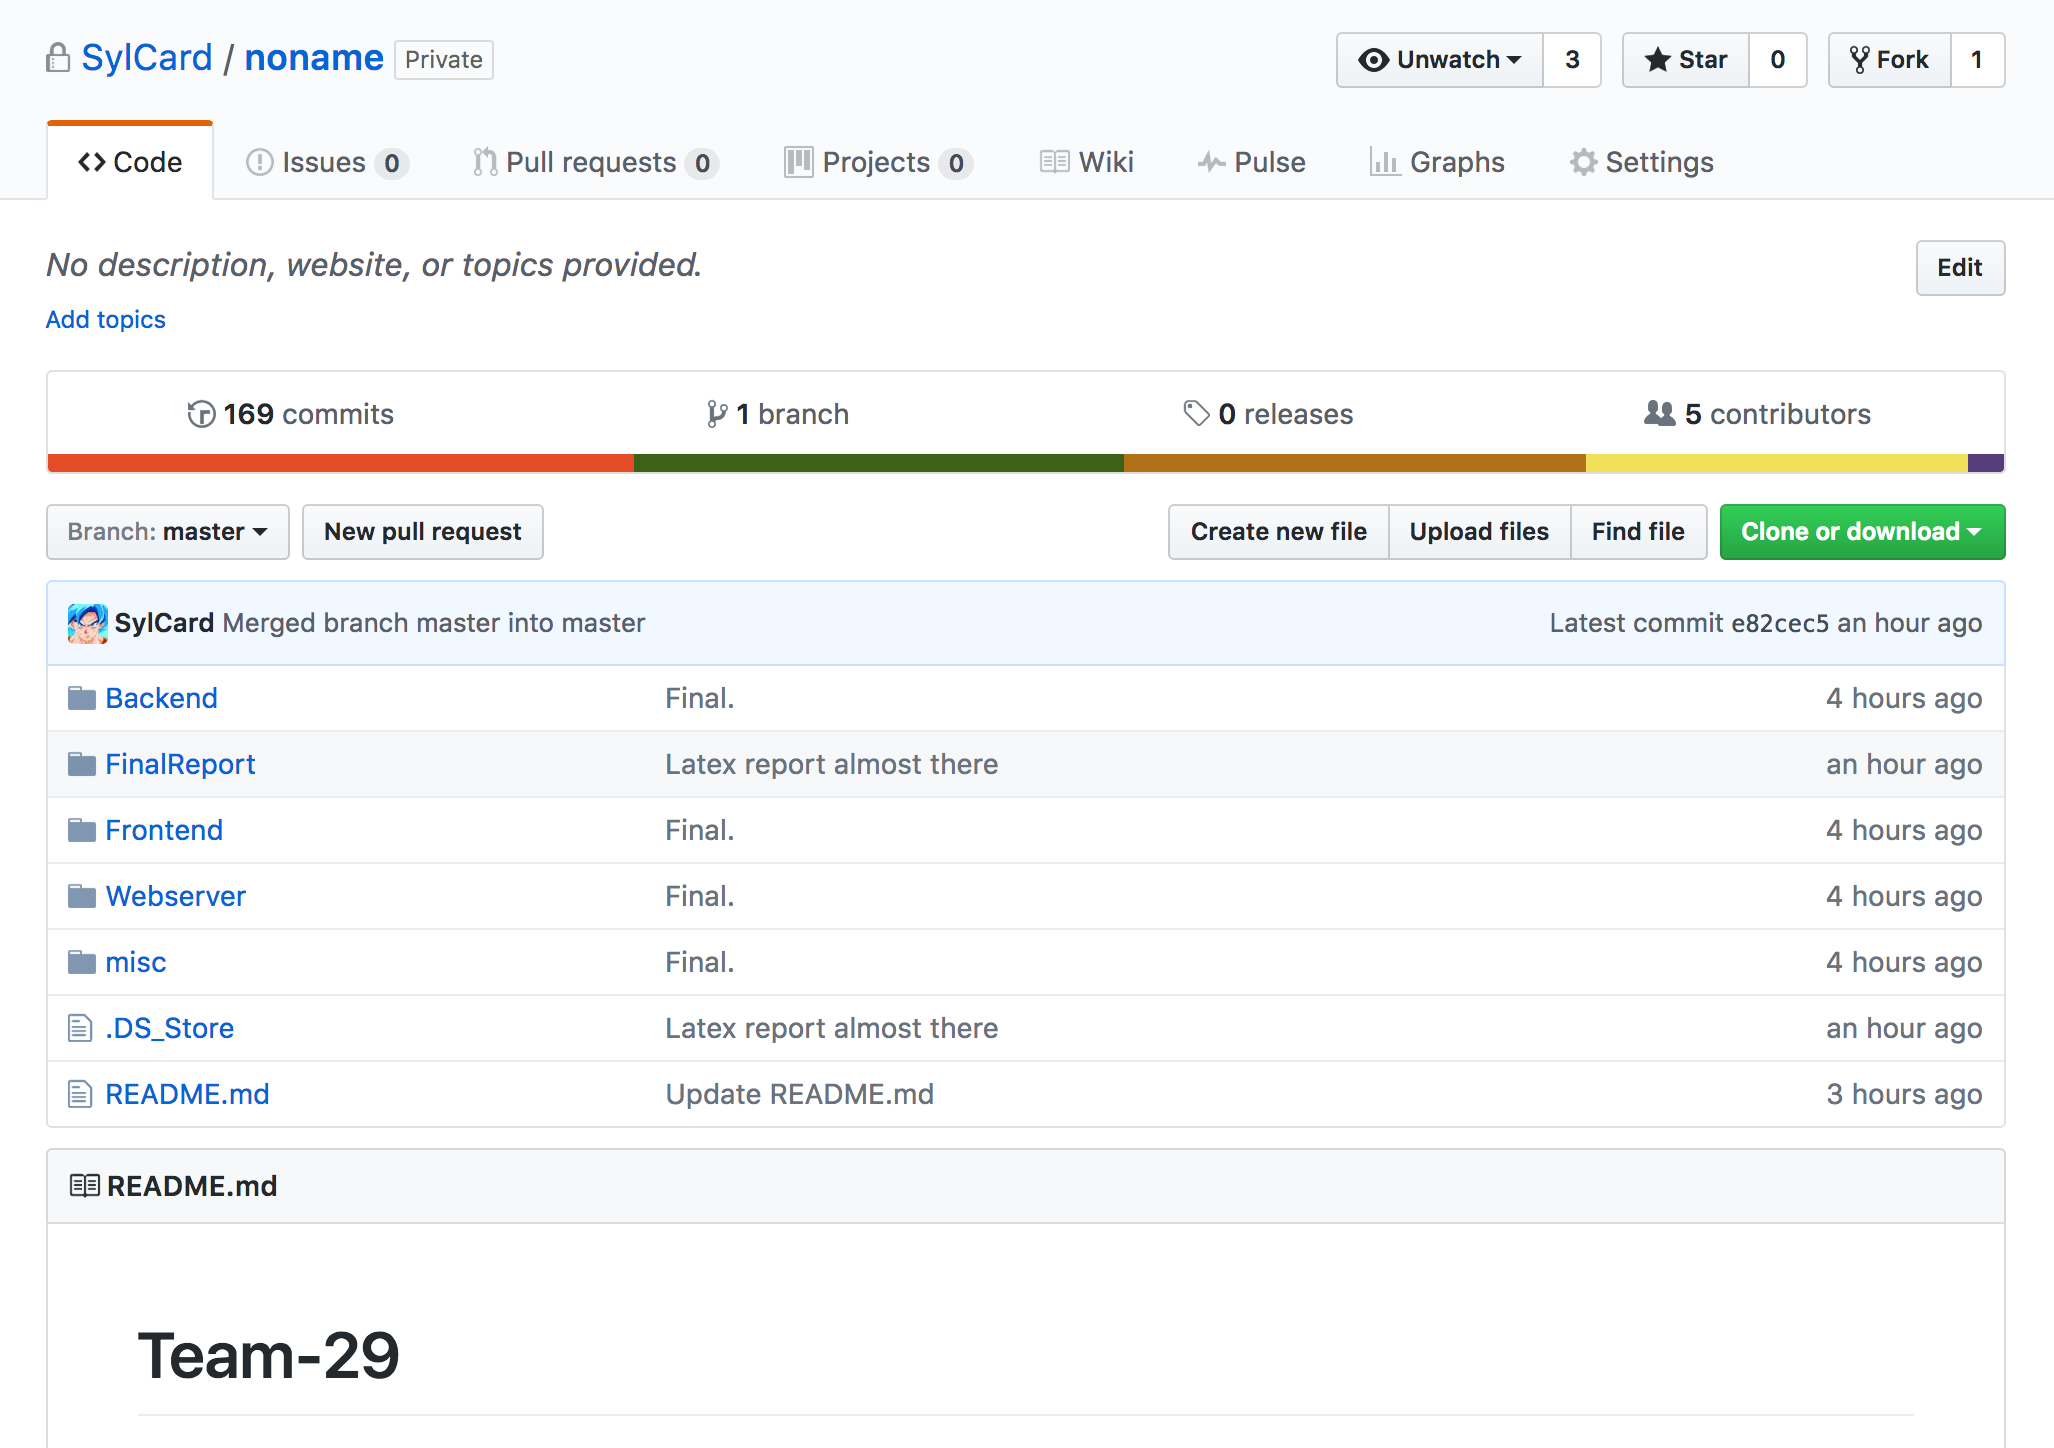
\includegraphics[width=120mm]{git.png}
  \caption{Shared Git Repository}
  \end{figure}
  \subsection{Roles}
  \textbf{Sylvester - Project Manager:}\newline
  Sylvester did an excellent job of allocating tasks to make sure everyone was always kept busy, and ensuring everyone was always on track regarding deadlines.
  He also arranged all of the meetings, made sure to book an appropriate study space for us to meet, and kept in regular contact with every team member on a daily basis.
  His great leadership was certainly a large contributor to the team’s success.
  \newline\newline\textbf{Tudor - Business Analyst:}\newline
  Tudor fufilled his role as business analyst to an astonishing degreee. He made major contributions to the Planning and Design document, taking the initiative to design and send mockups of the UI to the client.
  He often made sure to relay our progress to our mentor and make sure all our queries were answered. Throughout the development, Tudor was able to give a critical analysis on certain problems and
  the design of the interface. In addition to this, he took it upon himself to learn AngularJS as to provide support to the front-end team.
  \newline\newline\textbf{Joseph - Backend Developer/Architect:}\newline
  Joseph's programming skills was essentially the driving force of the project, through his major contributions to the backend we were able to lift our program concept from the whiteboard to the terminal.
  He frequently approached our mentor outside of 'official' meetings, to develop a much better grasp on how to build the best application for the client. Through Joseph's extensive testing we were able
  to progress our application further overcoming any obstacle.
  \newline\newline\textbf{Ollie - Backend Developer/Algorithms Developer:}\newline
  Ollie’s background in Maths and Statistics as a Data Science student helped him to produce the pivotal pseudocode algorithms for detecting  Volume Spikes, Fat Finger errors and Price Manipulation,
  which were then improved upon and coded with help from the rest of the team. He also contributed to the writing of the Planning and Design document as well as the Final Report.
  \newline\newline\textbf{Anil - Frontend Developer:}\newline
  With an in-depth knowledge of multiple frontend technologies including HTML, CSS and JavaScript, Anil was well equiped to work on the NodeJS interfaces.
  He setup our testing webserver and allowed us to see our changes live, which sped the testing process exponentially. He learnt how to use the Express framework
  and Socket.io.
  \newline\newline\textbf{Josh - Frontend Developer:}\newline
  Josh worked alongside Anil in the development of the frontend, helping to create the design of the user interface making it align with the principles of an outstanding UI.
  His research into graph libraries and contribution to data visualisation was wonderful.
  The efficiency and simplicity of the web application is a testament to how well Josh and Anil both worked together, and to what a great job they did.
\section{Evaluation}
Overall the system is robust and user friendly and as a team we are happy with the product. However, given more time we know that the functionality of the application could be increased to cover stretch goals not mentioned in the specification.
It is capable of handling large datasets in short periods of time, and due to it’s use of threading it can analyse data at the same time as it’s extracting it from it’s source.
Thanks to the simplistic UI the data is presented in a way that any non-technical user should be able to understand.
The system itself fulfills all the C-requirements set out in the specification. It learns the characteristics of stocks, in such a way as to allow detection of anomalies such as volume spikes, pump \& dumps and fat finger errors
It swiftly provides the user with alerts on unusual behaviour, including visualisation of the data and an option for further information.
\subsection{User Interface}
The user interface has continued along the lines of the planned version. It is simple and intuitive.
Each anomaly is clearly marked and contains enough data to inform the user of the situation around the anomaly, without presenting huge amounts of unnecessary information.
If the user interface was to be improved, this could be achieved by detailed user acceptance testing to create a truly bespoke application for the client
\subsection{System efficiency in handling of data}
Through various iterations the codes level of efficiency has been risen. To increase speed all data has been kept in memory for all checks.
Otherwise thanks to the simple design of the system it is capable of processing extraordinarily large amounts of data in short periods of time.
For example, the system can currently can process an average day's worth of data in 26 seconds.
\subsection{C-Requirements}
The development team set out to ensure that all requirements specified at the start of the project have been implemented according to the initial agreement.
Because development was based on the D-Requirements established, tests were carried out to verify that all C-Requirements have been satisfied in the process.
\begin{itemize}
  \item The system should be able to parse both real-time and historical data
      \begin{itemize}
        \item \textbf{PASS:} The system can successfully parse both real-time and historical data, detecting anomalies in both
      \end{itemize}
      \item Accept and Decline alerts flagged by the system. The system will adapt future alerts based on user input
      \begin{itemize}
            \item \textbf{PASS:} If the user deems an alert acceptable, the system will continue as normal.
            However, if the user declines an alert then the system will modify the sensitivity of the anomaly detection algorithm.
      \end{itemize}
      \item The program will be able to detect fat-finger errors in the data
      \begin{itemize}
        \item \textbf{PASS:} The system alerts the user when a fat finger is detected in the data
      \end{itemize}
      \item The program will be able to detect pump \& dump manipulation in the data
      \begin{itemize}
        \item \textbf{PASS:} The system alerts the user when pump \& dump is detected in the data
      \end{itemize}
      \item The system should be able to recognise normal market behaviour
      \begin{itemize}
        \item \textbf{PASS:} The application calculates exponential moving averages, to understand what normal behaviour is
      \end{itemize}
      \item The system should allow the user to see the cause of an alert
      \begin{itemize}
        \item \textbf{PASS:} Both the drop down arrow and the drill down provide the user with enough information to see why the anomaly was flagged
      \end{itemize}
      \item The system should be suitable for non-technical users
      \begin{itemize}
        \item \textbf{PASS:} The UI provides an elegant and simple design that requires minimal technical knowledge to operate
      \end{itemize}
      \item The system must be able to process large data sets and remain responsive
      \begin{itemize}
        \item \textbf{PASS:} Currently, the system can handle at least 100MB files and remain responsive, given sufficient storage it could withstand more.
      \end{itemize}
      \item The system must have a friendly user interface design
      \begin{itemize}
        \item \textbf{PASS:} With a simple colour scheme and a user-accepted design, the UI definitely fulfills this requirement
      \end{itemize}
\end{itemize}
\end{document}

% Content ends
